\section{Physical}
  \begin{frame}
    \frametitle{Aims}
      \begin{itemize}
        \item Interface data link layer,
        \item (De)Encode,
        \item Transmit: 1 after 0 (after 0 or 1, after 0... or 1)
      \end{itemize}
  \end{frame}
  \begin{frame}
    \frametitle{Hardware medium}
      \begin{itemize}
        \item IEEE 802.3 (a.k.a. Ethernet): $<$100Gbit/s
        \item IEEE 802.11 (a.k.a. Wi-Fi): $<$50 Mbit/s (802.11ad goes up to 6.75 Gbit/s)
        \item IEEE 802.15.1 (a.k.a. Bluetooth): $<$1 Mbit/s
        \item IEEE 802.15.4 (a.k.a. ZigBee): $<$250 kbit/s
        \item IEEE 802.16 (a.k.a. Wi-Max): $<$40 Mbit/s
        \item IEEE 1394 (a.k.a. Firewire): $<$3200 Mbit/s
        \item USB, serial port such as RS-232...
      \end{itemize}
  \end{frame}
  \begin{frame}
    \frametitle{Hardware medium: IEEE 802.3 (Ethernet)}
    \begin{figure}[t]
      \centering
      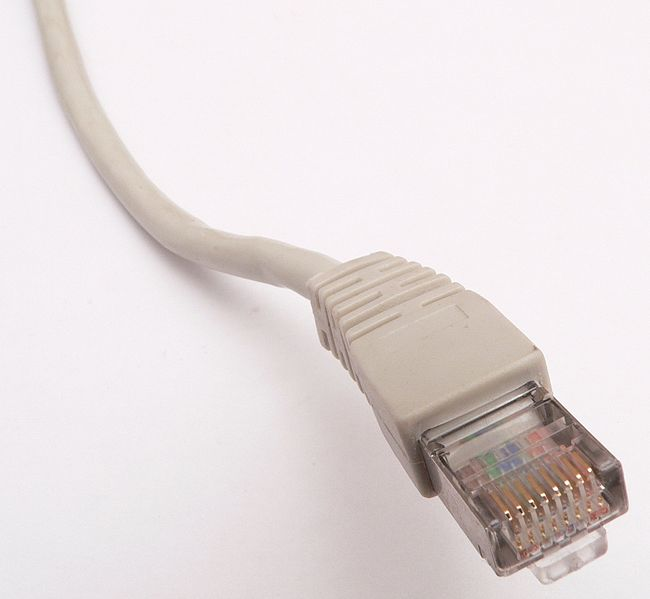
\includegraphics[height=5cm]{./imgs/rj45.jpg}
      \caption{\color{blue}\href{https://en.wikipedia.org/wiki/File:Ethernet_RJ45_connector_p1160054.jpg}{RJ45 connector}}
      \label{fig:rj45}
    \end{figure}
  \end{frame}
  \begin{frame}
    \frametitle{Hardware medium: IEEE 802.15.1 (Bluetooth)}
    \begin{figure}[t]
      \centering
      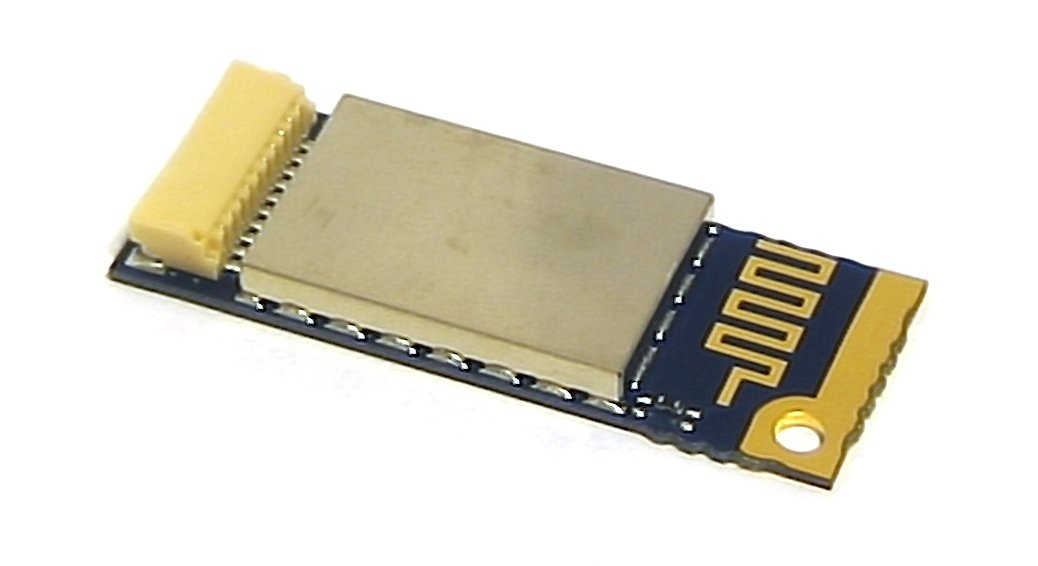
\includegraphics[height=5cm]{./imgs/bluetooth_card}
      \caption{\color{blue}\href{https://upload.wikimedia.org/wikipedia/commons/2/28/DELL_TrueMobile_350_Bluetooth_card.jpg}{Bluetooth card}}
      \label{fig:bluetooth_card}
    \end{figure}
  \end{frame}
  \begin{frame}
    \frametitle{Hardware medium: IEEE 802.15.4 (ZigBee)}
    \begin{figure}[t]
      \centering
      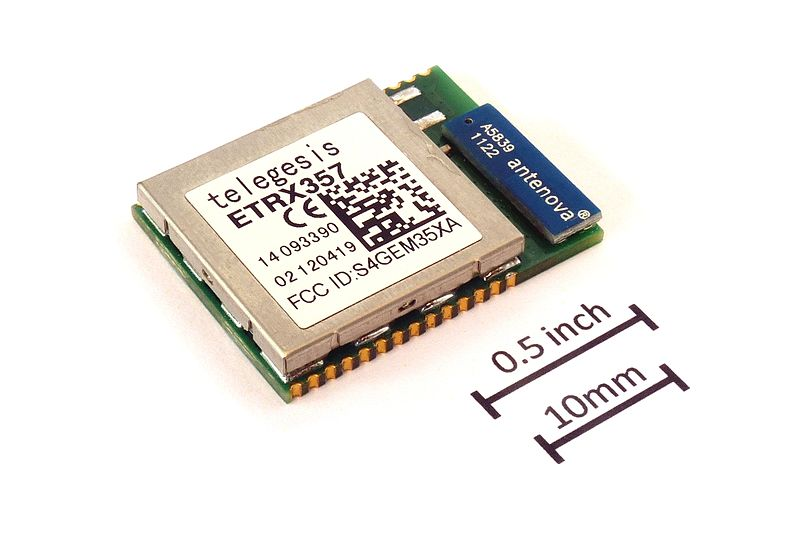
\includegraphics[height=5cm]{./imgs/zigbee.jpg}
      \caption{\color{blue}\href{https://upload.wikimedia.org/wikipedia/commons/thumb/2/29/ETRX357_ZigBee_module_with_size_ref.JPG/800px-ETRX357_ZigBee_module_with_size_ref.JPG}{ZigBee card}}
      \label{fig:ZigBee}
    \end{figure}
  \end{frame}
  \begin{frame}
    \frametitle{Hardware medium: IEEE 802.16 (Wi-Max)}
    \begin{figure}[t]
      \centering
      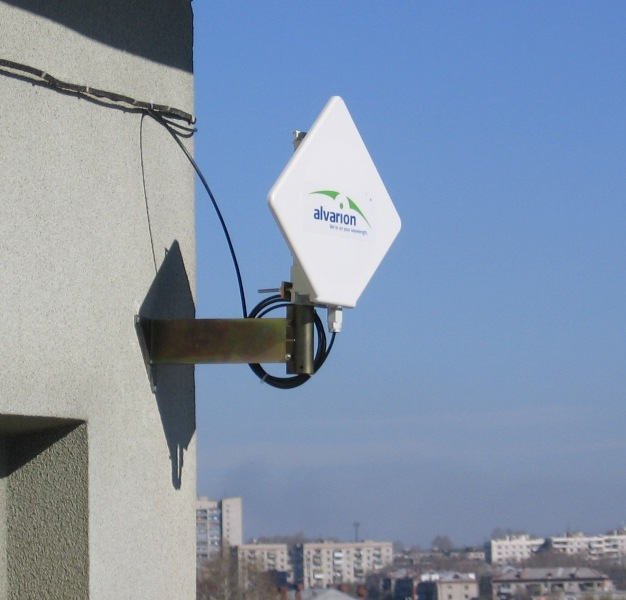
\includegraphics[height=5cm]{./imgs/Wi-Max.jpg}
      \caption{\color{blue}\href{https://upload.wikimedia.org/wikipedia/commons/d/db/Alvarion_CPE.jpg}{Wi-Max antenna}}
      \label{fig:Wi-Max_antenna}
    \end{figure}
  \end{frame}
  \begin{frame}
    \frametitle{Hardware medium: IEEE 1394 (Firewire)}
    \begin{figure}[t]
      \centering
      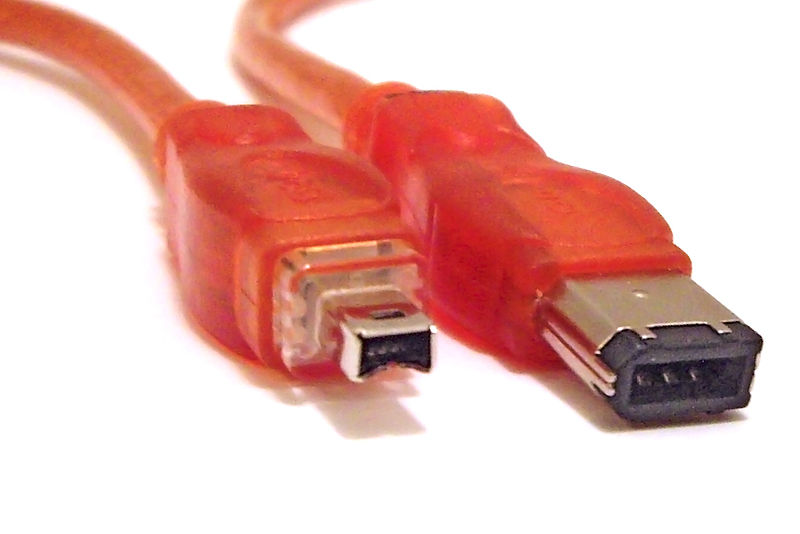
\includegraphics[height=5cm]{./imgs/firewire.jpg}
      \caption{\color{blue}\href{https://upload.wikimedia.org/wikipedia/commons/thumb/f/f7/FireWire_cables.jpg/800px-FireWire_cables.jpg}{Firewire connector}}
      \label{fig:firewire}
    \end{figure}
  \end{frame}
  \begin{frame}
    \frametitle{Encoding}
      \begin{itemize}
        \item \textbf{MLT3 (Multi-Level Transmit):} state changes for 1s over 3 levels, stays in the same state for 0s
        \item \textbf{AMI (Alternate Mark Inversion):} state 0 for 0s, state +/-1 for 1s
        \item \textbf{Manchester:} voltage transition (rising/falling edge mean 1/0)
        \item \textbf{BMC (Biphase Mark Code):} change its state for 1s, stay on the same state for 0s
        \item and so on...
      \end{itemize}
  \end{frame}
  \begin{frame}
    \frametitle{Encoding: Multi-Level Transmit}
    \begin{figure}[t]
      \centering
      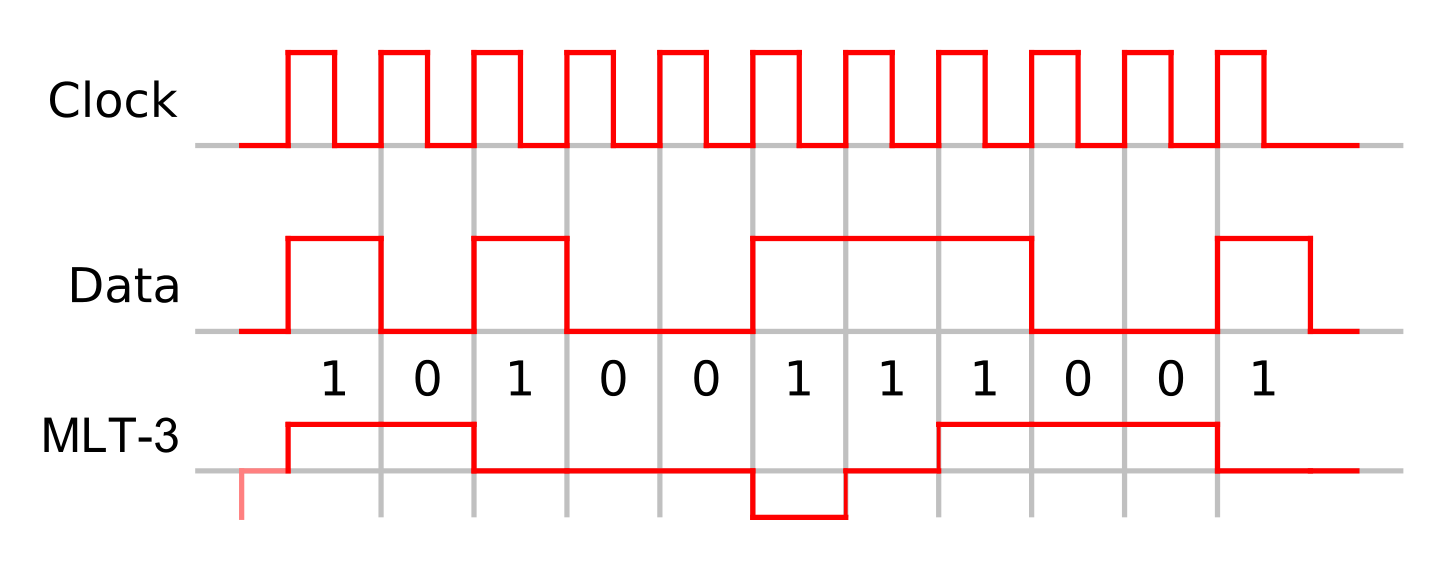
\includegraphics[height=3cm]{./imgs/mlt3.png}
      \caption{\color{blue}\href{https://upload.wikimedia.org/wikipedia/commons/thumb/b/b4/MLT3encoding.svg/1456px-MLT3encoding.svg.png}{Multi-Level Transmit}}
      \label{fig:mlt3}
    \end{figure}
  \end{frame}
  \begin{frame}
    \frametitle{Encoding: Alternate Mark Inversion}
    \begin{figure}[t]
      \centering
      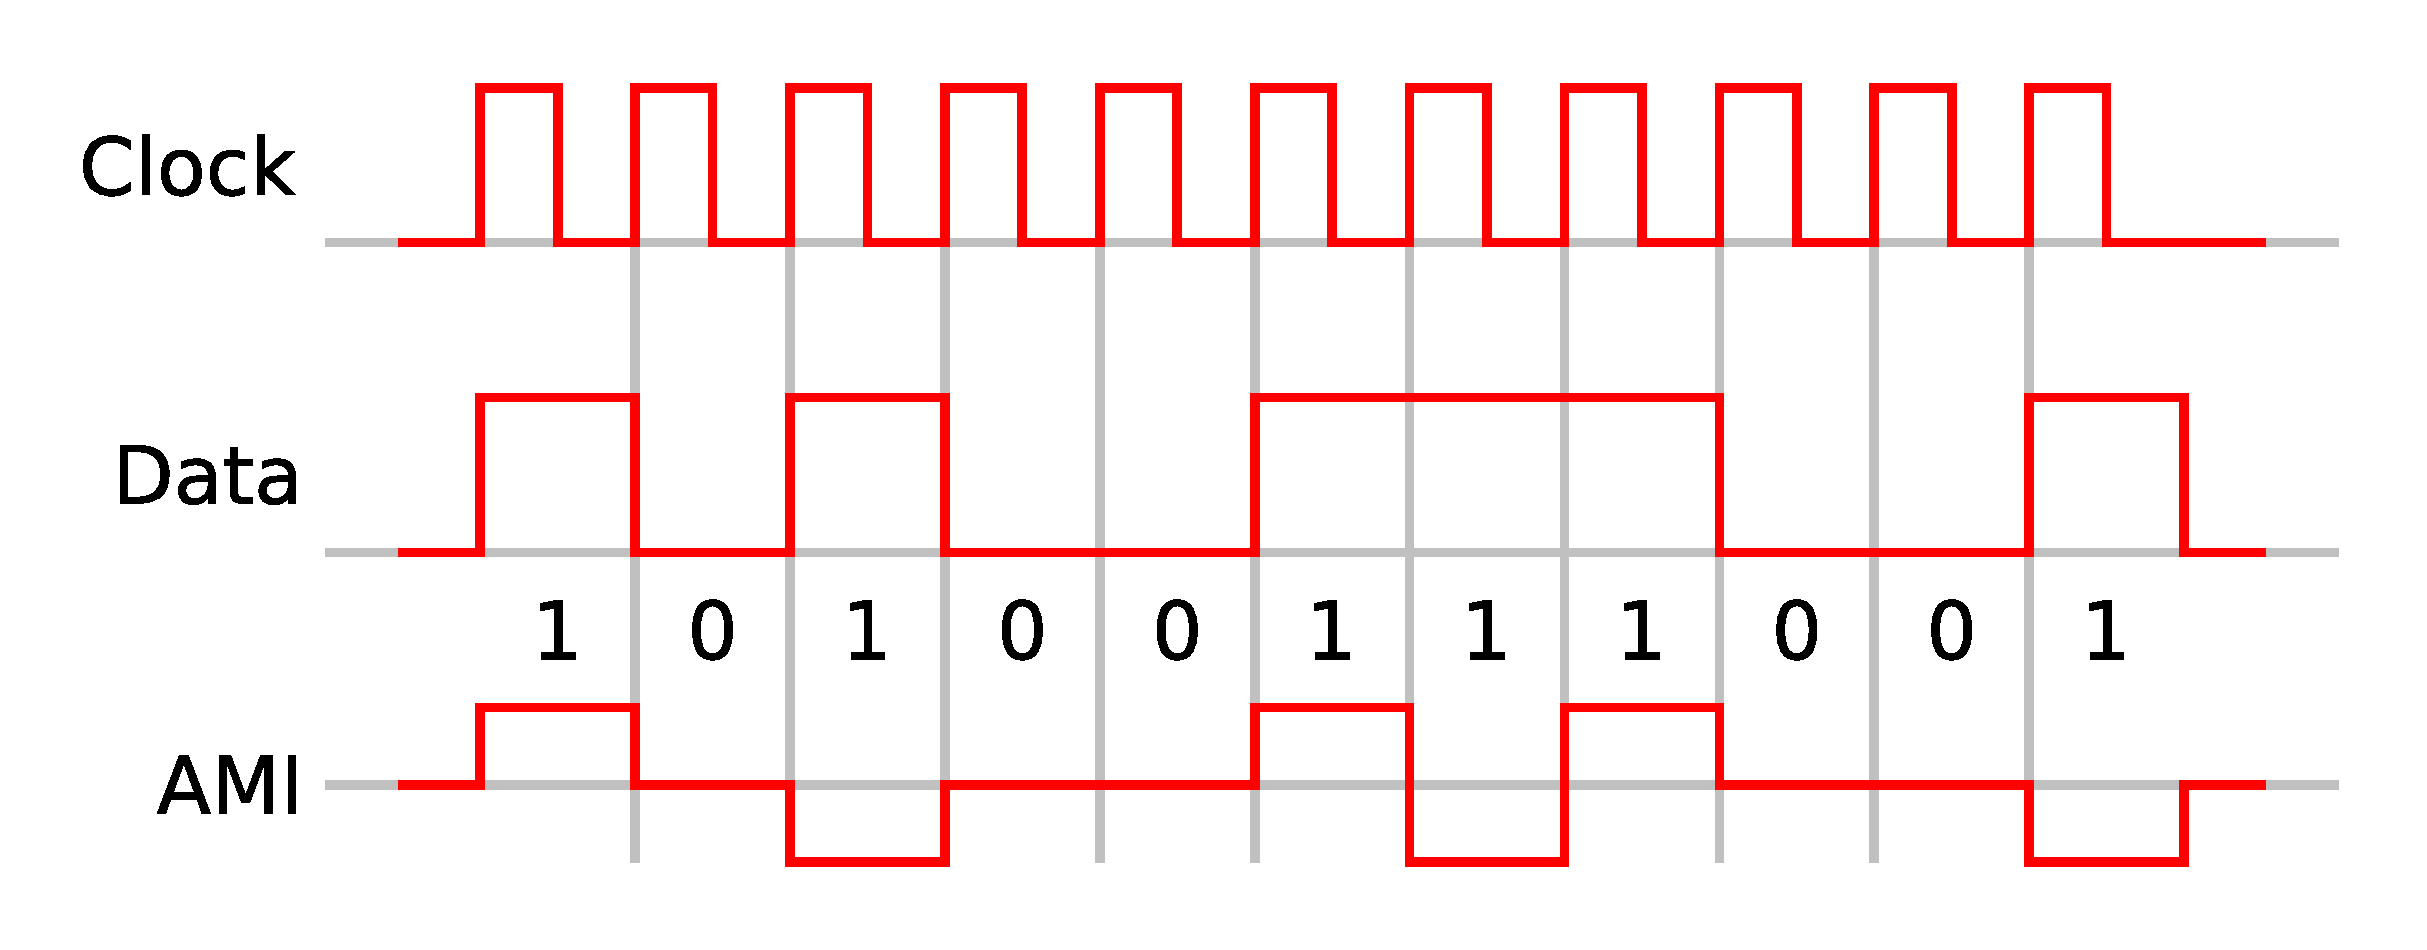
\includegraphics[height=3cm]{./imgs/ami.pdf}
      \caption{\color{blue}\href{https://upload.wikimedia.org/wikipedia/commons/b/b6/Ami_encoding.svg}{Alternate Mark Inversion}}
      \label{fig:ami}
    \end{figure}
  \end{frame}
  \begin{frame}
    \frametitle{Encoding: Manchester}
    \begin{figure}[t]
      \centering
      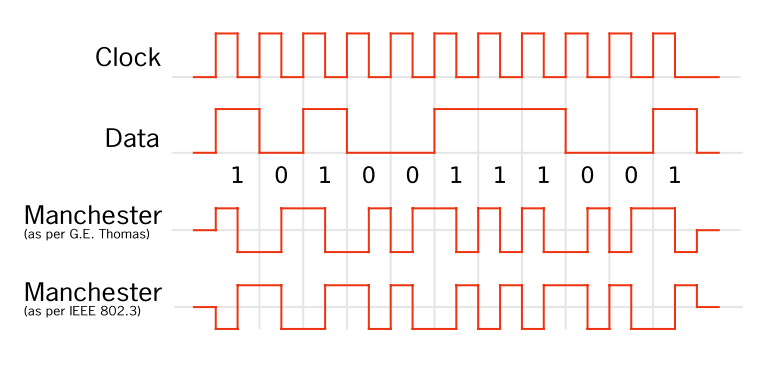
\includegraphics[height=3cm]{./imgs/manchester.png}
      \caption{\color{blue}\href{https://upload.wikimedia.org/wikipedia/commons/thumb/9/90/Manchester_encoding_both_conventions.svg/771px-Manchester_encoding_both_conventions.svg.png}{Manchester}}
      \label{fig:manchester}
    \end{figure}
  \end{frame}
  \begin{frame}
    \frametitle{Encoding: Biphase Mark Code}
    \begin{figure}[t]
      \centering
      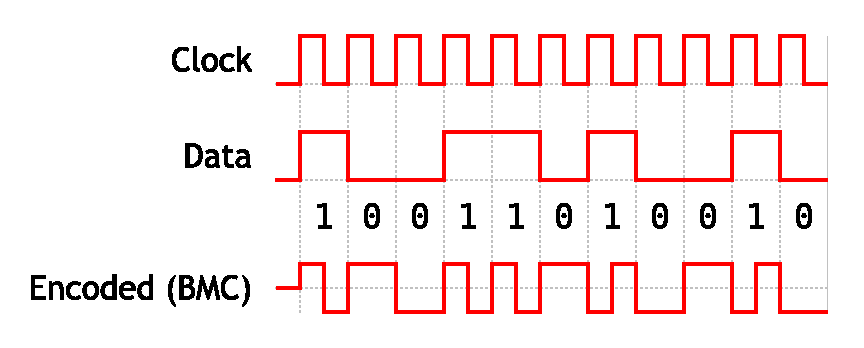
\includegraphics[height=3cm]{./imgs/bmc.pdf}
      \caption{\color{blue}\href{https://upload.wikimedia.org/wikipedia/commons/c/cb/Biphase_Mark_Code.svg}{Biphase Mark Code}}
      \label{fig:bmc}
    \end{figure}
  \end{frame}
  \begin{frame}
    \frametitle{Transmitting}
    \begin{figure}[t]
      \centering
      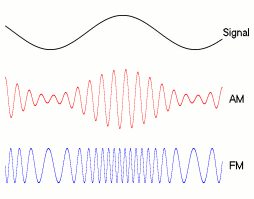
\includegraphics[height=5cm]{./imgs/modulation.png}
      \caption{\color{blue}\href{https://upload.wikimedia.org/wikipedia/commons/a/a4/Amfm3-en-de.gif}{Amplitude and phase modulation}}
      \label{fig:modulation}
    \end{figure}
  \end{frame}
  \begin{frame}
    \frametitle{Error detection}
      \begin{itemize}
        \item Repetition (hum...)
        \item Parity (XOR)
        \item Checksum
        \item CRC (Cyclic redundancy check): with a polynomial divison
        \item Hash
        \item and so on...
      \end{itemize}
  \end{frame}
  \begin{frame}
    \frametitle{Error correcting}
      \begin{itemize}
        \item Repetition (again)
        \item Hamming
        \item MDPC (Multidimensional parity-check code)
      \end{itemize}
  \end{frame}

  \begin{frame}
    \frametitle{Correction: MDPC}
    Raw data to send: 0x01 02 03 04
      \begin{figure}[h]
      \centering
      \begin{tabular}{cc|c}
        0x01 & 0x02 & 0x03 \\
        0x03 & 0x04 & 0x07 \\ \hline
        0x04 & 0x06 &
      \end{tabular}
      \caption{Data received with MDPC}
      \label{fig:ami}
    \end{figure}
  Data sent (with MDPC): 0x01 02 03 03 04 07 04 06
  \end{frame}
